这一节,我们讨论的UB,是由开发者指定应用于应用中的。要做到这一点,首先需要从不同的角度来考虑UB。 

到目前为止,我们看到的所有UB的例子都可以分为两种。第一类是像\texttt{++k +k}表达式这样的代码,这些都是错误,因为其根本没有定义行为。第二种是像\texttt{k + 1}这样的代码,其中\texttt{k}是有符号整数。这中代码到处都是,而且大多数时候,都工作得很好。除了变量为特定的某些值外,它的行为有良好的定义。

换句话说,代码具有隐式的先决条件:只要满足了这些先决条件,程序就会表现良好。请注意,在更大程序的上下文中,这些先决条件可能是隐式的,也可能不是:程序可能验证输入或中间结果,并防范可能导致UB的值。无论采用哪种方式,开发者都与用户有了一种约定:如果输入符合某些限制,则保证结果是正确的,并且程序可以以一种定义良好的方式运行。

如果违反了限制会发生什么?

那么就有以下两种可能:

\begin{itemize}
\item 
首先,程序可能检测到输入不符合约定,并处理错误。这种行为仍然得到了很好的定义,并且是规范的一部分。

\item 
其次,程序可能无法检测到约定被违反,并像往常一样继续进行。由于约定对于保证正确的结果至关重要,所以现在在一个未知的领域运行,而且没有办法预测将会发生什么。
\end{itemize}

这就是UB的描述。

既然我们已经理解了UB仅是在指定的约定之外运行的程序的行为,那么可以考虑一下如何将其应用到我们的应用中。

大多数足够复杂的程序在其输入上都有先决条件,即与用户进行约定。有人可能会说,应该总是检查这些先决条件,并报告错误。然而,这可能是一个非常昂贵的需求。让我们再来看一个例子。

我们想要编写一个程序来扫描画在一张纸上(或蚀刻在印刷电路板上)的图像,并将其转换为图形数据。程序的输入可能是这样的:

%\hspace*{\fill} \\ %插入空行
\begin{center}
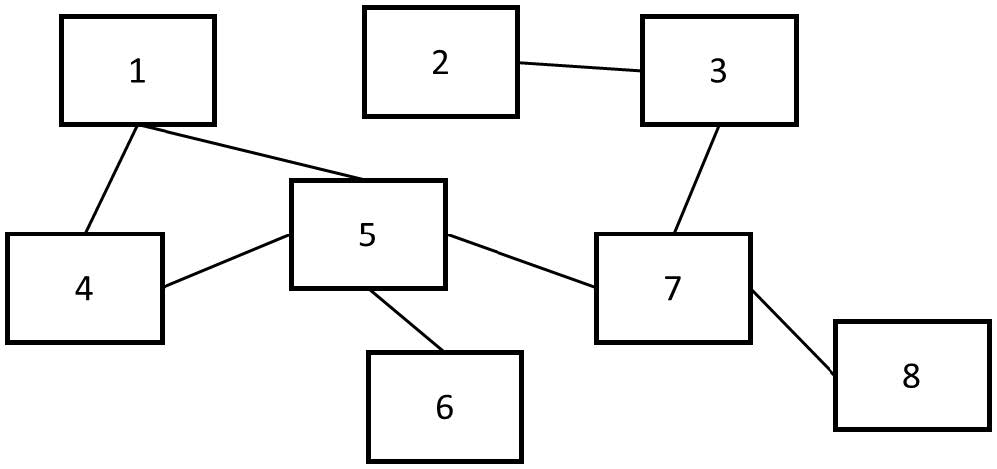
\includegraphics[width=0.9\textwidth]{content/3/chapter11/images/8.jpg}\\
图11.8 - 图形绘制是图形程序的输入
\end{center}

程序获取图像,识别矩形,从每个矩形创建图形节点,识别直线,为每条直线找出它连接的两个矩形,并在图形中创建相应的边。

假设我们有一个图像采集和分析库,为我们提供一组形状(矩形和直线)及其所有坐标,所以现在要做的就是找出哪些直线连接哪些矩形。有了所有的坐标,所以从现在开始,问题就是纯几何的。表示这个图最简单的方法之一是用边表表示。我们可以使用任何容器(比如,\texttt{vector})作为表,如果给每个节点分配一个唯一的数字ID,一条边就是一对数字。我们可以使用任意数量的几何算法来检测直线和矩形之间的交点,并逐边构造这个表(以及图本身)。

听起来很简单,我们有一个数据的自然表示,相当简单,并容易处理。不幸的是,我们还与用户有一个隐式约定:我们要求每条线恰好与两个矩形相交(同样,矩形也不互相相交,避免混乱)。 

%\hspace*{\fill} \\ %插入空行
\begin{center}
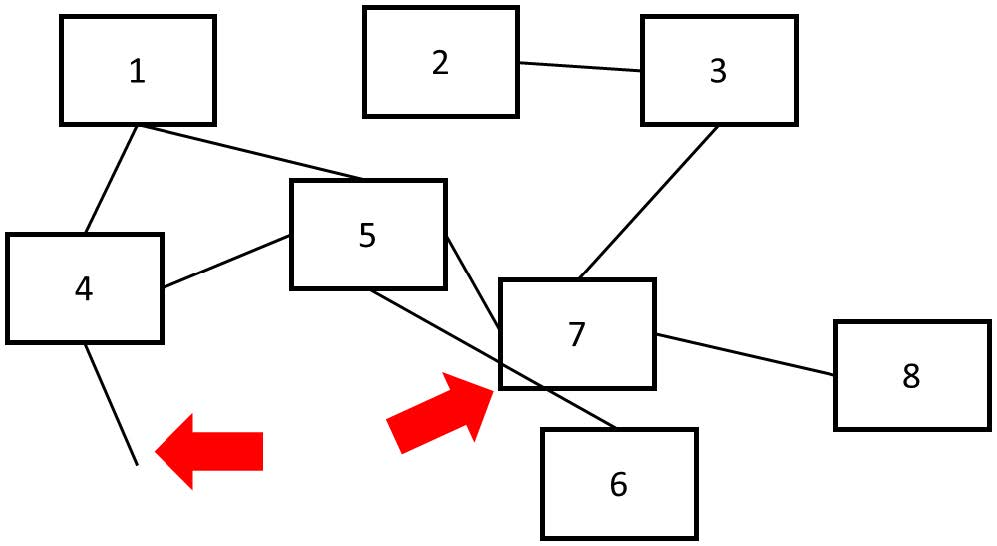
\includegraphics[width=0.9\textwidth]{content/3/chapter11/images/9.jpg}\\
图11.9 - 图形识别程序的无效输入
\end{center}

图11.9中,我们看到了一个违反约定的输入:其中一条线连接了三个矩形,而另一条线只连接了一个矩形。如前所述,我们有两个选择:可以检测并报告输入错误,或者可以忽略它们。第一个选项使我们的程序健壮,但带来了显著的性能损失:原始程序可能会在找到第二个这样的矩形后,停止寻找连接到给定边的矩形,并从那时起忽略这条边。这种优化的收益是相当可观的:对于类似于图11.8(但要大得多)的图,它可以将运行时间减少一半。如果输入最终是正确的,那么强制输入验证会浪费大量时间,并且会让有其他方法确保输入有效的用户感到沮丧。不验证输入将导致UB:如果有一条线连接三个矩形,算法将在找到前两个矩形后停止,无论它处理它们的顺序是什么(这个顺序可能是依赖于数据的,所以对于这种情况,可以说的是在涉及的两个节点之间将创建了一条边)。

如果性能差异不明显(或者总体运行时间很短,所以翻倍也不重要),那么最好的解决方案就很明显——验证输入。在这种情况和许多其他情况下,验证的成本很容易与找到解决方案一样高。在这种情况下应该怎么做呢?

首先,必须清楚强加给用户的约定。我们应该清楚地指定,并记录什么是有效的输入。在此之后,性能敏感型项目的最佳实践是提供最佳性能。更广泛的约定(施加更少限制的约顶)总是比狭义的约定好,所以如果有一些无效输入,我们可以很容易地检测,并以最小的开销处理它们,那么就应该这样做。除此之外,我们所能做的就是记录程序行为未定义时的条件,就像C++标准一样。 

还可以做一些额外的努力,可以为用户提供一个输入验证工具,既可以作为程序中的一个可选步骤,也可以作为单独的软件。运行它需要时间,但是如果用户从主程序中得到了奇怪的结果,可以使用工具检查,以确保输入是有效的。这比在行为未定义时简单地描述要好得多(然而,在有些情况下,这样的验证开销太大,反而不实用)。

如果C++编译器开发人员为我们做同样的工作,并提供一个可选的工具来检测代码中的UB,岂不妙哉?事实证明,开发人员也是这么想的:今天许多编译器都有一个选项来启用UB杀灭器(通常称为UBSan)。让我们从一些可以导致UB的代码开始了解其工作原理:

\begin{lstlisting}[style=styleCXX]
int g(int k) {
	return k + 10;
}

\end{lstlisting}

编写一个程序,用足够大的参数(大于\texttt{INT\_MAX-10})调用这个函数,并在启用UBSan的情况下编译它。对于Clang或GCC,该选项是\texttt{-fsanitize=undefined}。这里有一个例子:

\begin{tcblisting}{commandshell={}}
clang++ --std=c++17 –O3 –fsanitize=undefined ub.C
\end{tcblisting}

运行该程序,就会看到如下内容:

\begin{tcblisting}{commandshell={}}
ub.C:10:20: runtime error: signed integer overflow: 
        2147483645 + 10 cannot be represented in type 'int'
\end{tcblisting}

就像在我们的图形示例中一样,UB检测需要时间,并且会使程序变慢,所以这应该在测试和调试时去做的事情。让杀灭器运行常规回归测试的一部分,并认真对待报告的错误:虽然今天生成了正确的结果,但并不意味着下一个编译器不会生成一些非常不同的代码,并更改结果。

我们已经了解了UB,为什么它有时是一种必要的恶,以及如何利用它来提高性能。你翻过这一页之前,让我们回顾一下我们了解过的东西。

























